\documentclass{minimal}

\usepackage[compat=1.1.0]{tikz-feynman}

\usepackage{hyperref}
\usepackage[capitalize]{cleveref}

% \tikzfeynmanset{ fermion/.style = {
%    decoration={
%      markings,
%      mark=at position 0.5
%           with {\arrow[scale=1.2]{latex}}
%      },
%    postaction=decorate
%    }
% }

\begin{document}
\begin{equation}
    \label{exchange}
\mathcal{M} =
    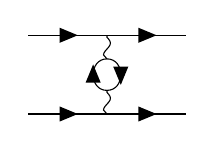
\begin{tikzpicture}[baseline=(c)]
        \begin{feynman}
            \vertex (a1) at (0, 0);
            \vertex (c1) at (2, 0);
            \vertex (a2) at (0, -1);
            \vertex (c2) at (2, -1);
            \vertex (x) at (1, 0);
            \vertex (l1) at (1, -.3);
            \vertex (c) at (1, -.5);
            \vertex (l2) at (1, -.7);
            \vertex (y) at (1, -1);
            \diagram*{
                {[edges=fermion]
                (a1) -- (x) -- (c1),
                (a2) -- (y) -- (c2),
                (l1) --[half left, looseness=1.5] (l2) --[half left, looseness=1.5] (l1),
                },
                {[edges=photon]
                (x) -- (l1),
                (l2) -- (y)
                }
            };
        \end{feynman}
    \end{tikzpicture}
\end{equation}



\begin{equation}
    \label{vacuum loop}
    \mathcal M =
    \feynmandiagram[small, baseline=(a)]{
        a [dot] --[fermion, out=130, in=230, min distance=2cm, looseness=1] a,
        a --[fermion, out=50, in=310, min distance=2cm, looseness=2] a,
    };
    \feynmandiagram[small, baseline=(a), horizontal=a to b]{
        a [dot] --[fermion, out=130, in=230, min distance=2cm, looseness=1] a,
        a -- [fermion, quarter right] b [dot] -- [fermion, quarter right] a,
        b --[fermion, out=50, in=310, min distance=2cm] b,
    };
\end{equation}

\begin{equation}
    \label{funckyyy}
    \feynmandiagram[small, horizontal=a to c]{
        a --[quarter left] b 
          --[quarter left] c 
          --[quarter left] d 
          --[quarter left] a,
        % a --[quarter left] b2 --[quarter left] c2 --[quarter left] d2 --[quarter left] a,
    };
    \feynmandiagram [horizontal=a to c] {
    a -- [red!0!blue, fermion, quarter left] b
      -- [red!33!blue, fermion, quarter left] c
      -- [red!66!blue, fermion, quarter left] d
        -- [red!100!blue, fermion, quarter left] a,
};
\end{equation}


\vspace{5cm}
\hspace{5cm}
aa
\begin{equation}
    \label{boop dee boop}
    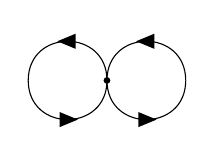
\begin{tikzpicture}[baseline=(c)]
        \begin{feynman}
            \vertex (a) at (0, 0);
            \vertex (b) at (1, 0);
            \vertex (c) at (2, 0);
            \filldraw[black] (b) circle (1pt);
            \diagram*{
                {[edges=fermion]
                (a)--[half right, looseness=1.7] (b)--[half right, looseness=1.7](a),
                (b)--[half right, looseness=1.7] (c)--[half right, looseness=1.7](b),
            }};
        \end{feynman}
    \end{tikzpicture}
\end{equation}
\begin{equation}
    \label{eq 1}
    F = ma
\end{equation}
\begin{equation}
    \label{eq 2}
    E = mc^2
\end{equation}
\begin{equation}
    \label{eq 3}
    a^2+b^2 = c^2
\end{equation}

% \feynmandiagram[horizontal=a to b, baseline=(c)]{
%     a --[fermion, half right, looseness=1.7] b[dot] --[fermion, half right, looseness=1.7] a,
%     b --[fermion, half right, looseness=1.7] c --[fermion, half right, looseness=1.7] b,
%     };

Mine diagram er \cref{exchange,boop dee boop,funckyyy,vacuum loop,eq 2,eq 3}.


\end{document}